\documentclass[a4paper,UKenglish,cleveref, autoref, thm-restate]{lipics-v2021}
%for section-numbered lemmas etc., use "numberwithinsect"
%for enabling thm-restate support, use "thm-restate"

\pdfoutput=1 %uncomment to ensure pdflatex processing (mandatatory e.g. to submit to arXiv)
\hideLIPIcs  %uncomment to remove references to LIPIcs series (logo, DOI, ...), e.g. when preparing a pre-final version to be uploaded to arXiv or another public repository

\graphicspath{{./fig/}}%helpful if your graphic files are in another directory

\bibliographystyle{plainurl}% the mandatory bibstyle

\title{PACE Solver Description: OCMu64,\\ a solver for One-sided Crossing Minimization} %TODO Please add

%\titlerunning{Dummy short title} %TODO optional, please use if title is longer than one line

\author{Ragnar {Groot Koerkamp}}{ETH Zurich, Switzerland}{ragnar.grootkoerkamp@gmail.com}{https://orcid.org/0000-0002-2091-1237}{}%TODO mandatory, please use full name; only 1 author per \author macro; first two parameters are mandatory, other parameters can be empty. Please provide at least the name of the affiliation and the country. The full address is optional. Use additional curly braces to indicate the correct name splitting when the last name consists of multiple name parts.

\author{Mees de Vries}{Unaffiliated, The Netherlands}{meesdevries@protonmail.com}{}{}

\authorrunning{R. Groot Koerkamp and M. de Vries} %TODO mandatory. First: Use abbreviated first/middle names. Second (only in severe cases): Use first author plus 'et al.'

\Copyright{Ragnar Groot Koerkamp and Mees de Vries} %TODO mandatory, please use full first names. LIPIcs license is "CC-BY";  http://creativecommons.org/licenses/by/3.0/

\ccsdesc[500]{Theory of computation~Mathematical optimization}
\ccsdesc[300]{Theory of computation~Computational geometry}

\keywords{Graph drawing, crossing number, branch and bound} %TODO mandatory; please add comma-separated list of keywords

\category{} %optional, e.g. invited paper

%% \relatedversion{\url{https://doi.org/10.5281/zenodo.11671980}} %optional, e.g. full version hosted on arXiv, HAL, or other respository/website
%\relatedversiondetails[linktext={opt. text shown instead of the URL}, cite=DBLP:books/mk/GrayR93]{Classification (e.g. Full Version, Extended Version, Previous Version}{URL to related version} %linktext and cite are optional

\supplement{}%optional, e.g. related research data, source code, ... hosted on a repository like zenodo, figshare, GitHub, ...
\supplementdetails[subcategory={Source Code}]{Software}{https://github.com/mjdv/ocmu64} %linktext, cite, and subcategory are optional
\supplementdetails[subcategory={Source Code}]{Software}{https://doi.org/10.5281/zenodo.11671980} %linktext, cite, and subcategory are optional

%\funding{(Optional) general funding statement \dots}%optional, to capture a funding statement, which applies to all authors. Please enter author specific funding statements as fifth argument of the \author macro.

%% \acknowledgements{I want to thank \dots}%optional

\nolinenumbers %uncomment to disable line numbering



%Editor-only macros:: begin (do not touch as author)%%%%%%%%%%%%%%%%%%%%%%%%%%%%%%%%%%
%% \EventEditors{John Q. Open and Joan R. Access}
%% \EventNoEds{2}
%% \EventLongTitle{42nd Conference on Very Important Topics (CVIT 2016)}
%% \EventShortTitle{CVIT 2016}
%% \EventAcronym{CVIT}
%% \EventYear{2016}
%% \EventDate{December 24--27, 2016}
%% \EventLocation{Little Whinging, United Kingdom}
%% \EventLogo{}
%% \SeriesVolume{42}
%% \ArticleNo{23}
%%%%%%%%%%%%%%%%%%%%%%%%%%%%%%%%%%%%%%%%%%%%%%%%%%%%%%

\newcommand{\R}{\mathbb R}
\renewcommand{\b}{\prec}
\newcommand{\be}{\preceq}
\newcommand{\g}{\bullet}
\renewcommand{\u}{\overline{u}}
\renewcommand{\v}{\overline{v}}
\DeclareMathOperator{\supp}{supp}

\begin{document}

\maketitle

%TODO mandatory: add short abstract of the document
\begin{abstract}
  Given a bipartite graph $(A,B)$, the \emph{one-sided crossing minimization}
  (OCM) problem is to find an ordering of the vertices of $B$ that minimizes the
  number of edge crossings when drawn in the plane.

  We introduce the novel \emph{strongly fixed}, \emph{practically fixed}, and
  \emph{practically glued} reductions that maximally generalize some existing
  reductions.
  We apply these in our exact solver OCMu64, that directly uses branch-and-bound
  on the ordering of the vertices of $B$ and does not depend on ILP or SAT
  solvers.
\end{abstract}

\section{Introduction}

The 2024 edition of PACE, an annual optimization challenge, considers the
\emph{one-sided crossing minimization} problem, defined as follows.
Given is a bipartite graph $(A, B)$ that is drawn in the plane at points
$(i, 1)$ and $(j,0)$ for components $A$ and $B$ respectively. The ordering of $A$
is fixed, and the goal is the find an ordering of $B$ that minimizes the number of
crossings when edges are drawn as straight lines.

We introduce some new reductions and give an overview of our algorithm. Proofs are brief or
omitted due to lack of space.

\section{Definitions}
We use $<$ to compare vertices in $A$ in their fixed ordering. We generalize to weighted graphs
for the proof of \cref{lem:sfp}: a node $u \in B$ is taken to be a function $u: A \to \mathbb
R^{\geq 0}$, where weight 0 represents an absent edge. We write $W_u = \sum_{a \in A}u(a)$ for
the total weight of $u$, and set $\bar u = u/W_u$. Write $N(u) = \supp(u) \subseteq A$ for the
set of neighbors of $u$.

We write $c(u, v) = \sum_{(a, b) \in A^2}
u(a)v(b)[a > b]$; in the unweighted case, this is the \emph{crossing number}, the number of
crossings between edges incident to $u$ and $v$ when $u$ is drawn before $v$.  For
$X,Y\subseteq B$ we set $c(X,Y) = \sum_{x\in X}\sum_{y\in Y} c(x,y)$ for the cost of ordering
all vertices of $X$ before all vertices of $Y$. More generally, $c(X,Y,Z) = c(X, Y) + c(X, Z) +
c(Y, Z)$. We also consider the \emph{reduced cost} $r(X,Y) = c(X, Y) - c(Y, X)$, which is
negative when $X$ is better \emph{before} $Y$ and positive when $X$ is better \emph{after} $Y$.

We write $u\b v$ when $u$ must come before $v$ in all minimal solutions, and say that $(u, v)$
is a \emph{fixed} pair.

\begin{figure}[t]
\centering
\hfill
\subfloat[An instance of \cref{lem:weak}.]{
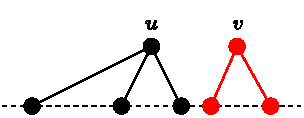
\includegraphics[width=0.30\textwidth]{fig/simple.pdf}%
\label{fig:simple}
}
\hfill
\subfloat[Examples of blocking sets (\cref{pfp}) in blue.]{
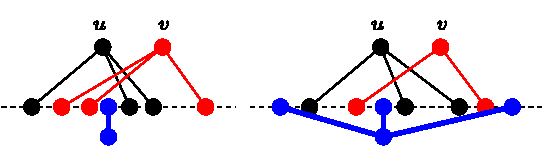
\includegraphics[width=0.6\textwidth]{fig/blocking-set.pdf}%
\label{fig:blocking}
}
\hfill
\\
\subfloat[Examples of strongly fixed pairs (\cref{def:sfp}).]{
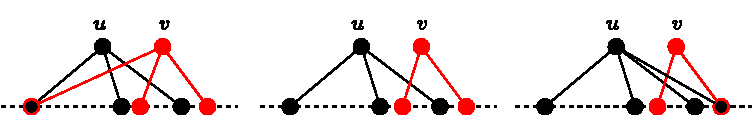
\includegraphics[width=0.9\textwidth]{fig/strongly-fixed.pdf}%
\label{fig:strongly-fixed}
}
%% \subfloat[]{
%% 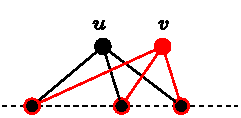
\includegraphics[width=0.33\textwidth]{fig/gluing.pdf}%
%% \label{fig:gluing}
%% }
\caption{
  Various examples where $u\b v$, where $u,v\in B$ can freely move around and
  their neighbours in $A$ (on the dashed line) have fixed positions.}%
\label{fig}
\end{figure}

\section{Methods}
\subsection{Reductions}
\subparagraph{Fixed pairs}
To reduce the search space of all possible orderings of $B$, it is crucial to automatically
find as many fixed pairs in $B$ as possible. Ideally, one would be able to determine whether $u
\b v$ by inspecting only $u, v$. For example, the following result, shown in \cref{fig:simple} is well known \cite[Lemma
  1]{dujmovic_2004}, RR1 of \cite{dujmovic_2008}.

% TODO: Citation
\begin{observation}\label{lem:weak}
  Let $u, v \in B$. When $\max N(u) \leq \min N(v)$ and $\bar u\neq \bar v$, then $u\b v$.
\end{observation}

We give a much stronger version of \cref{lem:weak}, with some examples in \cref{fig:strongly-fixed}. In fact, \cref{lem:sfp} is the strongest
generalization possible when only considering $u$ and $v$ themselves, without further inspection of
$A$ or the other elements of $B$ (see \cref{rem:strongest}). This also generalizes RR3 of
\cite{dujmovic_2008}.

\begin{definition}[Strongly fixed pair]\label{def:sfp}
    We call $u, v \in B$ a \emph{strongly fixed pair} if for every $b \in A$ we have ${\sum_{a
    \leq b} \bar u(a) \geq \sum_{a \leq b} \bar v(a)}$, and at least one of these inequalities
    is strict. Note that this implies $r(u, v) < 0$.
\end{definition}
\begin{lemma}\label{lem:sfp} When $u, v$ is a strongly fixed pair,
    then for any $w: A\to \mathbb R^{\geq 0}$ we have 
    \[
        r(w, \bar v) \leq r(w, \bar u).
    \]
\end{lemma}
\begin{proof}
    Consider the least element $a_0 \in A$ such that $\bar u(a_0) \neq
    \bar v(a_0)$. We must have $\bar u(a_0) > \bar v(a_0)$. Now consider the transformation of
    $\bar u$ which ``moves'' $\delta := \bar u(a_0) - \bar v(a_0)$ of weight from $a_0$ to its
    successor $a_1 \in A$, and call this transformed function $\bar u'$. Then
    \[
        r(w, \bar u') = r(w, \bar u) - \delta w(a_0) - \delta w(a_1) \leq r(w, \bar u).
    \]
    Since $\bar v$ is obtained from $\bar u$ by a sequence of such transformations,
    the inequality follows.
\end{proof}
\begin{lemma}\label{lem:sfimplf}
    If $(u, v)$ is strongly fixed, then $u \b v$.
\end{lemma}
\begin{proof}
    Suppose towards a contradiction that $v < x_0 < \cdots < x_k < u$ is part of an optimal
    solution. Write $X = \sum_i x_i$ for the combined function. Then by assumption $r(X, u)
    \leq 0$, and therefore $r(X, v) = W_v r(X, \bar v) \leq W_v r(X, \bar u) = W_v / W_u \cdot
    r(X, u) \leq 0$. But then $c(X, u, v) < c(X, v, u)\leq c(v, X, u)$, which
    contradicts $(v,X,u)$ being optimal.
\end{proof}

\begin{remark}
    Consider $u \neq v$ from the original, unweighted problem, taking only values $0, 1$. Let 
    $n = |N(u)|, m = |N(v)|$, and consider both as ordered lists. Then $u, v$ are strongly
    fixed if and only if for all $0 \leq i < n$, $N(u)_i \leq N(v)_{\lfloor i\cdot m/n
    \rfloor}$ and at least one of the inequalities is strict, which is how we check in practice
    whether $u, v$ is strongly fixed.
\end{remark}

\begin{remark}\label{rem:strongest}
    By inspecting only $u, v$, it is not possible to do better than \cref{lem:sfimplf}. If $u,
    v$ with $\bar u \neq \bar v$ are not strongly fixed, and we can assume the existence of any
    additional nodes in $A, B$, then we can conjure a situation where $v \b u$.

    Suppose that $b \in A$ be some element such that $U := \sum_{a \leq b} \bar u(a) < \sum_{a \leq
    b} \bar v(a) =: V$, and take $M \in A$ to be some element between $b$ and its succesor. Also,
    take $L < \min(N(v))$ and $R > \max(N(u))$. Now consider a new element $X \in B$, which
    connects only to $L, M, R$. We claim that by picking the right weights for $X$, we can
    obtain $c(v, X, u) < \min(c(X, u, v), c(u, v, X))$, which establishes that in the presence
    of $X$, $v \b u$.

    We have that
    \[
        c(X, u, v) - c(v, X, u) = r(u, v) + W_v(2VX(M) + X(R) - X(L) - X(M))
    \]
    and
    \[
        c(u, v, X) - c(v, X, u) = r(u, v) + W_u(X(L) + (1-U)X(M) - X(R) - UX(M)),
    \]
    and if we can choose $X(L), X(M), X(R)$ so that both these values are positive, we are
    done. We can always scale these values up, so we can ignore the $r(u, v)$ term in both
    equations; we can also ignore $W_u, W_v$. Because we can choose $X(R), X(L)$ as we please,
    it suffices if the sum of the remaining pairs of expressions, which is
    \[
        (2V - 1)X(M) - (2U - 1)X(M),
    \]
    is positive. But indeed it is, since by assumption $U < V$.

    Suppose that $u, v \in B$ with $\bar u \neq \bar v$ are not strongly fixed, and let $b \in
    A$ be some element such
    that $\sum_{a \leq b} \bar u(a) > \sum_{a \leq b} \bar v(a)$. By taking $X: A \to \mathbb
    R^{\geq 0}$ some function which assigns very high
    weight to $b$, we can obtain $c(v, X, u) < \min(c(X, u, v), c(u, v, X))$, showing that
    \cref{lem:sfp} is optimal.
\end{remark}
Although such a function $X$ may exist in theory, it does
not have to exist in the actual set $B$, motivating the following definition
that generalizes RRLO2 of \cite{dujmovic_2008}.

\begin{lemma}\label{pfp}
  Suppose $r(u,v)< 0$.
    A \emph{blocking set} $X\subseteq B-\{u,v\}$ is a set such that $c(v,X,u) \leq \min(c(v, u,
    X), (X, v, u))$.  If there is no blocking set for $(u, v)$, we call it a
    \emph{practically fixed pair}, and $u\b v$.
\end{lemma}

In practice, such a blocking set $X$ can be found, if one exists, using a knapsack-like algorithm: for
each $x\in B-\{u,v\}$, add a point $P_x = (r(v, x), r(x, u))$, and search for a subset summing
to ${\leq{}(r(u, v), r(u, v))}$. \cref{fig:blocking} shows some examples.

Note that we do not require $(v, X, u)$ to be a true local minimum, since we do
not consider interactions between vertices in $X$, as that would make ruling out the
existence of such sets much harder.

\begin{remark}[Weak variants]
  It is also possible to consider \emph{weak} variants of the above lemmas that
  only imply that $u < v$ in \emph{some} optimal solution. This requires careful
  handling of cycles like $u\be v\be w\be u$.
\end{remark}

\subparagraph{Gluing}
We now turn our attention to \emph{gluing}, i.e., proving that two vertices $u$
and $v$ always go right next to each other, and we can treat them as a single vertex. First,
let us see that we cannot get `strong gluing' result analogous to \cref{lem:sfimplf}.

\begin{remark}
  When $N(u)=N(v)$ in the unweighted case, or more generally $\bar u=\bar v$, we can glue $u$
    and $v$.
  Otherwise when $r(u,v)\leq 0$, there is an $X : A\to \mathbb R^{\geq 0}$ such that $(u, X, v)$ is
  strictly better than $(u,v,X)$ and $(X,u,v)$.
\end{remark}
\begin{lemma}[Practical gluing]\label{pg}
    Let $u$ and $v$ satisfy $r(u, v) \leq 0$.
    A non-empty subset $X\subseteq B-\{u,v\}$ is \emph{blocking} when $c(u, X, v) \leq
    \min(c(u, v, X), c(X, u, v))$. If there is no blocking set, then we can glue $u, v$.
\end{lemma}
Again such sets $X$ can be found or proven to not exist using a knapsack
algorithm: add points $P_x = (r(u, x), r(x, v))$ and search for a non-empty
set summing to $\leq{}(0,0)$.

Let us also mention this gluing-like reduction: \emph{gluing to the front}, implied by RRL01 of
\cite{dujmovic_2008}.
\begin{lemma}[Greedy]\label{greedy}
  When $r(u, x)\leq 0$ for all $x\in B$, there is a solution that
  starts with $u$.
\end{lemma}

\begin{remark}[Tail variants]
  Our branch-and-bound method fixes vertices of the
solution from left to right. Thus, at each step \cref{pg,pfp} can be applied to
just the \emph{tail}.
\end{remark}


\subsection{Branch-and-bound}
Our solver \texttt{OCMu64} is based on a standard branch-and-bound on the ordering of the
solution.  We start with fixed prefix $P=()$ and tail $T=B$, and in each step we try (a
subset of) all vertices in $T$ as the next vertex appended to $P$.
In a preprocessing step we compute the trivial lower bound $S_0 =
\sum_{u,v}\min(c(u,v),c(v,u))$ on the score.
We keep track of the score $S_P$ of the prefix and $S_{PT}=c(P, T)$ of
prefix-tail intersections, and abort when this score goes above the best
solution found so far. The \emph{excess} of a tail is its optimal score minus
the trivial lower bound. We do a number of optimizations.

\begin{description}
  \item[Graph simplification] We drop degree-$0$ vertices, merge identical
    vertices, and split the graph into \emph{independent} components
    \cite[Corollary 2]{dujmovic_2004} when
    possible. We find an initial solution using the median heuristic \cite{eades_median,eades_median_2} and a local search that tries to move
    slices and optimally insert them \cite{makinen_experiments,eades_heuristics}, and re-label all nodes accordingly to make
    memory accesses more efficient.
  \item[Fixed pairs] We find all strongly fixed pairs and store them. For the
    exact track we also find practically fixed pairs. Instances for the parameterized
    track are simple enough that the overhead was not worth it. Also for each
    tail we search for new `tail-local' practically fixed pairs. In each state, we only
    try vertices $u\in T$ not fixed by another $v\in T$.
  \item[Gluing] We use the greedy strategy of \cref{greedy}. Our implementation
    of \cref{pg} contained a bug, so we did not use this. (Also benefits
    seemed limited.)
  \item[Tail cache] In each step, we search for the longest suffix of $T$ that
    was seen before, and reuse (the lower bound on) its excess. We also
    cache the tail-local practically fixed pairs.
  \item[Optimal insert] Instead of simply appending $u$ to $P$, we
    insert it in the optimal position. Note that the
    implementation is tricky because it interacts in complicated ways with
    the caching of results for each tail.
\end{description}

\newpage

\bibliography{bibliography}

\end{document}
